\documentclass[12pt, a4paper]{article}
\usepackage[spanish,activeacute]{babel}
\usepackage[utf8]{inputenc}
\usepackage[T1]{fontenc}
\usepackage{helvet} % Importando helvética
\renewcommand*\familydefault{\sfdefault} % Arial

\usepackage{apacite}
\usepackage{natbib} % Natbib

\usepackage{geometry}
\newgeometry{bottom=2.5cm, top=4cm, left=2.5cm, right=2.5cm}

\usepackage{ragged2e}
\renewcommand{\baselinestretch}{1.25}
\setlength{\parindent}{0pt}
\setlength{\parskip}{6mm}

\setlength{\skip\footins}{1.5cm}
\setlength{\footnotesep}{0.5cm}

\usepackage{graphicx}
\usepackage[font=small,labelfont=bf]{caption}
\usepackage[skip=0pt]{subcaption} \captionsetup[subfigure]{labelformat=empty}
\usepackage{float}
\usepackage{booktabs}
\usepackage[dvipsnames]{xcolor}

\usepackage{amsmath}

\usepackage[colorlinks = True, linkcolor = blue, urlcolor = blue, citecolor = blue]{hyperref}
\usepackage{xurl}


%%%%%%%%%%%%%%%%%%%%%%%%%%%%%%%%%%%%%%%%%%%%%%%%%%%%%%%%%%%%%%%%%%%%%%%%%%%%%%%%%%%%%%%%%%%%

\title{Análisis de sentimientos en comentarios de Among Us}
\author{Mauricio Alvarado}
\subtitle{Reporte}
\date{\today}


%%%%%%%%%%%%%%%%%%%%%%%%%%%%%%%%%%%%%%%%%%%%%%%%%%%%%%%%%%%%%%%%%%%%%%%%%%%%%%%%%%%%%%%%%%%%
% Referencias/Bibliografía

%\usepackage[babel]{csquotes}
%\usepackage[backend=biber,style=apa]{biblatex}
%\renewcommand*{\bibfont}{\normalfont\scriptsize} % Cambiar tamaño del texto
%\setlength\bibitemsep{1.5\itemsep} % Separación entre cada referencia
%\DeclareLanguageMapping{spanish}{spanish-apa}
%\addbibresource{<<ruta>>} % Importando biblio
%\nocite{*} % Incluir las que no se citó

% Dentro del main se debe colocar: \printbibliography
% https://tex.stackexchange.com/questions/131518/help-with-citation-in-text-in-parentheses-etc-with-biblatex-apa

%%%%%%%%%%%%%%%%%%%%%%%%%%%%%%%%%%%%%%%%%%%%%%%%%%%%%%%%%%%%%%%%%%%%%%%%%%%%%%%%%%%%%%%%%%%%
% Paquetes adicionales:___________________________________________________
% Para tablas complejas se puede usar la página: https://www.tablesgenerator.com/
% Para cortar tablas, el paquete: \usepackage{multicol}
% Para tablas que abarcan más de dos páginas: \usepackage{longtable}
% Para páginas rotar páginas, sin rotar en enunciado: \usepackage{pdflscape}, usar comando: {landscape}
% Colores de fondos, textos, entre otros: \usepackage{color}
% Para cargar imágenes de pdfs: \usepackage{pdfpages}



% Recursos:
% Como datos de entrenamiento se usará el dataset traducido del corpus Stanford Sentiment
% Treebank (SST-2). El dataset se puede acceder desde  el siguiente url:
% https://huggingface.co/datasets/mrm8488/sst2-es-mt

\begin{document}
\maketitle


\section{Motivación}
% Explicar el app
\textit{Among Us} es un videojuego multijugador en línea desarrollado por la compañía estadounidense \textit{InnerSloth}. Fue lanzado en 2018 con poco recibimiento. No obstante, el juego alcanzó una enorme popularidad en 2020 durante la pandemia de COVID-19, convirtiéndose en uno de los juegos más jugados del año.

La historia de \textit{Among Us} se desarrolla en una nave espacial, donde los jugadores asumen el papel de miembros de la tripulación o impostores que intentan sabotear la misión. Los jugadores trabajan juntos para mantener la nave en funcionamiento mientras completan tareas, pero algunos jugadores son impostores cuyo objetivo es sabotear y matar a los demás jugadores sin ser descubiertos. A medida que los jugadores completan tareas, también investigan los asesinatos y acusan a otros jugadores de ser los impostores. Estos deben utilizar la estrategia y la comunicación para determinar quién es el impostor y votar para expulsarlo de la nave.

% Motivo para escogerlo
Pese a que el juego aún cuenta con mucha popularidad y recibió muchas mejoras de parte de los desarrolladores, durante los primeros meses de la pandemia el juego contaba con muchos errores y caídas en sus servidores debido a la alta demanda. Esto llevó a muchas personas a calificar el juego de manera negativa. Actualmente cuenta con una calificación de 3.8 en \textit{Google Play Store}, lo cual lo posiciona muy por debajo de muchos juegos de igual o menor popularidad. Por ello, lo que motiva a este proyecto es poder clasificar los comentarios de un juego muy popular y de mis favoritos del 2020, que actualmente ha solucionado gran parte de sus problemas, pero que aún cuenta con una calificación muy baja.

% Rango de fechas de los comentarios
Se tomará en cuenta los cinco mil comentarios más actuales en castellano y en Perú. La última actualización es considerando los comentarios hasta la fecha de 22 de febrero del 2023.


\section{Metodología}

\subsection{Modelos}
Se consideraron un algoritmo de \textit{machine learning} (\textit{ML}) y dos  arquitecturas neuronales de \textit{deep learning} (\textit{DL}). Cada uno corresponde a un modelo, por lo que se estimó 3 modelos diferentes.

El algoritmo considerado para \textit{ML} es el de Regresión Logística. Fue elegido por ser uno de los algoritmos más usados para propuestas simples de clasificación. De hecho, es uno de los primeros algoritmos que se aprenden en diversos cursos a lo largo del mundo. Se estimó la mejor versión de este basado en la selección de los hiperpárametros que maximicen el ajuste con los datos de entrenamiento. Se usó el método \textit{GridSearchCV} que recoge las diferentes combinaciones de hiperparámetros definidos con anterioridad y estima el modelo con 5-Folds mediante \textit{cross-validation}\footnote{Consiste en separar las observaciones de entrenamiento en cinco grupos, estimar con cuatro de estos y reservar el quinto como un \textit{testing} para estimar el ajuste. Tras realizar este ejercicio con las cinco combinaciones posibles, se obtiene cinco métricas de ajuste diferentes que serán promediadas. El objetivo de este ejercicio es corroborar la inexistencia de \textit{overfitting}, lo cual se debería reflejar en métricas de ajuste en los datos de \textit{test} muy similares al de los de entrenamiento.}. Entre las diferentes alternativas se consideró como parámetros de regularización a 0.001, 0.01, 0.1, 1, 10 y 100.

Para el caso los algoritmos de \textit{DL}, se propuso dos arquitecturas neuronales que cuentan con capas de \textit{embedding}, \textit{convolucionales}, \textit{dropout}, \textit{pooling} y \textit{densas}. La primera estructura será llamada “Básica” y la segunda será llamada “Intermedia”. La primera se divide por las siguientes capas:
\begin{itemize}
	\itemsep0em 
	\item Embedding: 15 000 dimensiones en el vocabulario
	\item Convolucional: 32 núcleos
	\item Pooling: Máximo global
	\item Dropout: 80\%
	\item Densa: 16 neuronas
	\item Densa: 1 neurona
\end{itemize}

Mientras que la segunda por lo siguiente:
\begin{itemize}
	\itemsep0em 
	\item Embedding: 15 000 dimensiones en el vocabulario
	\item Convolucional: 64 núcleos
	\item Pooling: Máximo global
	\item Dropout: 30\%
	\item Densa: 128 neuronas
	\item Densa: 64 neuronas
	\item Densa: 1 neurona	
\end{itemize}

En el entrenamiento se tomará en cuenta que todas las observaciones deben ser tokenizadas y no debe existir \textit{stopwords}. En particular, para el modelo de Regresión Logística se aplicará una lematización al dataset previo a la vectorización vía TF-IDF. En cambio, para el caso de los modelos de redes neuronales se vectorizará directamente mediante el método \textit{Tokenizer} de \textit{keras}. Esto debido a que las observaciones no deben ser lematizadas en las redes neuronales si se cuenta con la capa Embedding, debido a que esta buscará relaciones entre las palabras. Este proceso puede alterarse y perder valor si se lematiza.

Como comentario final, que se retomará en la subsección 3.2, todos estos modelos se estimarán con el dataset traducido del Corpus Stanford Sentiment Treebank (SST-2). El mejor modelo será el seleccionado para clasificar los comentarios de \textit{Among Us} en la \textit{Google Play Store}.


\subsection{Comparativa entre modelos}
\subsubsection{\textit{Log-Loss}}
Medida de la calidad de predicción de un modelo de clasificación, donde se evalúa la distancia entre las probabilidades de predicción y las etiquetas verdaderas. También se le conoce como “función de pérdida”, por su traducción al castellano. Se define por lo siguiente:
\begin{equation}
	Log-Loss = - \dfrac{1}{N} \sum_{i=1}^{N} y_i * log(p) + (1-y_i) * log (1-p)
\end{equation}
donde $p$ es la probabilidad de clasificar como $1$. Los valores de $Log-Loss$ varían entre 0 y $\infty$, donde un valor de 0 indica una predicción perfecta. En ese sentido, en la medida que un algoritmo asigne una menor función de pérdida, será preferido ante otro.

\subsubsection{F1-score}
Medida de combina la precisión (\textit{precision}) y la exhaustividad (\textit{recall}) de un modelo de clasificación. Dado que la precisión se define por:
\begin{equation}
	precision = \dfrac{Verdadero\ positivo}{Verdadero\ positivo + Falso\ positivo}
\end{equation}
y la exhaustividad por:
\begin{equation}
	recall = \dfrac{Verdadero\ positivo}{Verdadero\ positivo + Falso\ negativo}
\end{equation}
El F1-score es la media armónica de ambos:
\begin{equation}
	F1-score = 2 \dfrac{precision * recall}{precision + recall}
\end{equation}
El $F1-score$ se sitúa entre 0 y 1, donde un valor de 1 indica una predicción perfecta.

\subsubsection{Curva \textit{Receiver Operating Characteristic} (ROC)}
Métrica para evaluar la calidad de un modelo de clasificación binaria. La curva ROC representa la tasa de verdaderos positivos frente a la tasa de falsos positivos para diferentes umbrales de probabilidad. Dada la cantidad de aciertos del total de verdaderos, la sensibilidad:
\begin{equation}
	sensibilidad = \dfrac{Verdadero\ positivo}{Verdadero\ positivo + Falso\ negativo}
\end{equation}
y la cantidad de aciertos del total de falsos, la especificidad:
\begin{equation}
	especificidad = \dfrac{Verdadero\ negativo}{Verdadero\ negativo + Falso\ positivo}
\end{equation}
La curva ROC se grafica con 1-Especificidad en el eje de las abscisas y la Sensibilidad en el eje de las ordenadas. En la medida que el área debajo de la curva sea mayor, el modelo cuenta con mayor potencia para distinguir entre los verdaderos y falsos bajo diferentes umbrales. Es importante notar que a medida que se buscar acertar más los verdaderos o falsos, se pierde la potencia en alguno de los dos, por lo tanto es un trade-off para cada umbral. Aquel modelo que cuente con mayor potencia es el preferido.


\section{Resultados}
\subsection{Datos}
Dado que no se cuenta con una categoría para los comentarios del juego \textit{Among Us} en la \textit{Google Play Store}; es decir, que la clasificación se realizará a “ciegas” sin saber si alguno de los algoritmos ha asignado los comentarios de manera correcta o no; es necesario primero entrenarlo con datos en los que sí se cuente con esta división.

Por ello, los tres algoritmos fueron estimados con el \textit{dataset} traducido del Corpus Stanford Sentiment Treebank (SST-2)\footnote{Disponible en: \url{https://huggingface.co/datasets/mrm8488/sst2-es-mt}.}. Este Corpus está basado en el trabajo de Pang y Lee (2005), en el que se recolectó 11.855 oraciones individuales de \textit{reviews} de películas. En Stanford se analizó y categorizó más de 215 mil frases únicas entre comentarios positivos y negativos. Para este proyecto se usará la versión traducida de dicho trabajo.

Tras haber entrenado y comparado los resultados entre los modelos, se usará este para clasificar los comentarios del juego \textit{Among Us} de la \textit{Google Play Store} extraídos hasta la fecha de 22 de febrero del 2023.

\subsection{Selección de modelo}
% Explicar el proceso del entrenamiento y de las pruebas (porqué escogieron esos
% algoritmos, qué métricas usaron y sus valores, cual obtuvo el mejor performance,
% problemas que se presentaron, etc.)
Tras la estimación de los modelos, se seleccionó el modelo de Regresión Logística con un parámetro de regularización de 10. Hacia adelante, este modelo será el comparado con las métricas de las dos redes neuronales. Para los tres modelos, se usó la predicción con los datos de testeo y con sus verdaderas asignaciones (etiquetas).

El Cuadro 1 muestra los resultados de las métricas de $Log-Loss$ y $F1-score$. Sorpresivamente, el modelo de Regresión Logística es aquel que presenta el mejor valor en la función de pérdida y también la que muestra mayor ajuste mediante la métrica de $F1-score$. Es sorpresivo debido a ser el modelo más simple entre las tres alternativas. Este resultado se podría explicar a varios factores, entre ellos al criterio diferenciado que se consideró en los modelos, donde a la regresión logística se aplicó lematización y no a las redes neuronales. No obstante, también puede deberse las redes neuronales contaron con \textit{overfitting} durante el proceso de estimación, lo cuál pese a varios experimentos no se logró reducir. Las Figuras se pueden encontrar al final del documento.

\begin{table}[htbp]
	\centering
	\caption{Métricas para cada modelo}
	\scalebox{0.8}{
	\begin{tabular}{lrr}
		Modelo & $Log-Loss$ & $F1-score$ \\
		\midrule
		Reg. Logística & \textbf{7.367} & \textbf{0.800} \\
		\midrule
		CNN Intermedia & 9.387 & 0.707 \\
		\midrule
		CNN Básica & 10.378 & 0.655 \\
	\end{tabular}%
	}
	\label{tab:addlabel}%
\end{table}%

La Figura 1 muestra las curvas ROC para diferentes umbrales. Se encuentra un resultado consistente con las anteriores métricas, en el que la Regresión Logística nuevamente es superior a las dos propuestas de arquitecturas neuronales. En este sentido, el modelo de simple de $ML$, con el hiperparámetro de 10 en la regularización resulta ser el mejor no solo entre sus diferentes alternativas, sino también entre los diferentes modelos propuestos para el entrenamiento-testeo. Este modelo es el seleccionado con el que se clasificará los comentarios de \textit{Among Us}.

\begin{figure}[h!]
	\centering
	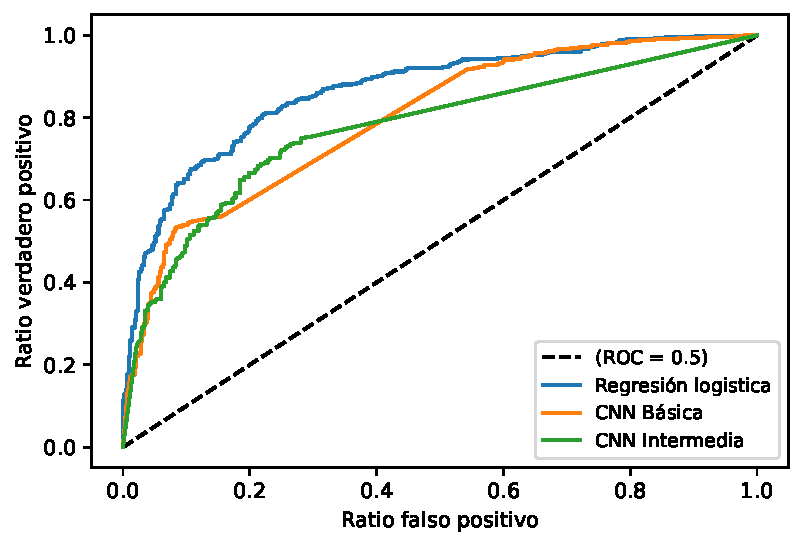
\includegraphics[width=0.6\textwidth]{../Figuras/roc.pdf}
	\caption{Curvas ROC}
\end{figure}

\subsection{Hechos estilizados}
% Indicar estadísticas (total de comentarios, cantidad de símbolos y palabras)
% Identificar cantidad de verbos y adjetivos en los comentarios
% Frecuencia de palabras condicional (por score)
En esta subsección se hará una revisión de las estadísticas de la base de datos de los comentarios de \text{Among Us}. Las principales estadísticas son las siguientes:
\begin{itemize}
	\itemsep0em 
	\item Total de observaciones: 5 000
	\item Total de palabras: 38 227
	\item Total de observaciones por \textit{score}: 1 (1 085), 2 (240), 3 (389), 4 (511), 5 (2 775)
	\item Total de palabras por \textit{score}: 1 (9 472), 2 (2 701), 3 (4 808), 4 (5 737), 5 (15 509)
	\item Cantidad de verbos: 9 921
	\item Cantidad de adjetivos: 8 582
\end{itemize}

La mayor cantidad de comentarios, como es de esperarse, se encuentra en los extremos. Finalmente, no se pudo identificar correctamente cuáles son las personas u organizaciones más mencionadas en los comentarios: varias palabras que son asignadas como estas no lo son realmente. Los que efectivamente sí son palabras u organizaciones son:
% ¿Qué personas u organizaciones son mencionados en los comentarios? (Top 3 personas más mencionadas)
\begin{itemize}
	\itemsep0em 
	\item Among Us: 54
	\item Google: 7
	\item Messi: 4
\end{itemize}


\subsection{Clasificación de comentarios}
% Brindar conclusiones
Con el modelo de clasificación elegido, la Regresión Logística, se procedió a predecir qué comentarios son positivos o negativos.

Como no se puede comparar el etiquetado con alguna referencia, debido a que este no existe, se comparó el etiquetado con el \textit{score}. Es razonable esperar que un comentario positivo esté acompañado de una calificación alta, y por el contrario, un comentario negativo lo esté con una calificación baja. De esta manera, el análisis debería enfocarse principalmente en los comentarios con los \textit{scores} que se encuentran en los extremos. 

Según la Figura 2, el modelo parece ser capaz de predecir con mucha certeza los comentarios positivos. Los comentarios con \textit{score} entre 2-4 los predice casi a la mitad de manera positiva y a la otra de manera negativa. Esto puede deberse a que estos cuenten con una fragmento del comentario que es positiva y otra que es negativa, propio de un comentario que no es calificado de manera categórica como un 1 o un 5. No obstante, para el caso extremo de negativo, el 1, el modelo no parece ser tan contundente al clasificar los comentarios como negativos. Se etiquetó a 656 comentarios como negativos y 429 como positivos, lo cual genera mucha incertidumbre.
\begin{figure}[h!]
	\centering
	\includegraphics[width=0.6\textwidth]{../Figuras/clasificación.pdf}
	\caption{Distribución de clasificación dado el \textit{score}}
\end{figure}


\section{Conclusiones}
A modo de conclusión se encontró que un modelo simple de Regresión Logística superó a las dos propuestas de redes neuronales en el proceso de entrenamiento con el \textit{dataset} traducido del Corpus Stanford Sentiment Treebank (SST-2). El resultado es consistente en los tres criterios de comparación: \textit{Log-Loss}, \textit{F1-score} y la curva ROC. 

Luego, en la clasificación de los \textit{Among Us} de la \textit{Google Play Store}, el modelo es capaz de clasificar los comentarios positivos de manera muy acertada. Esto tomando en consideración que estos comentarios positivos deberían ser congruentes con un \textit{score} alto. Por el contrario, el modelo parece ser inexacto para clasificar comentarios negativos.

Queda en agenda aumentar más algoritmos de clasificación como el Decision Tree, Random Forest, XGBoost y SVM. Además, se debe mejorar las arquitecturas de redes neuronales de tal manera que se encuentre una que no genere \textit{overfitting}. Tomando esto en consideración, se espera reducir la incertidumbre en la clasificación de comentarios muy negativos y positivos.

\begin{thebibliography}{99}
	
\bibitem {} Pang, B., y Lee, L. (2005). Seeing Stars: Exploiting Class Relationships for Sentiment Categorization with Respect to Rating Scales. \textit{arXiv preprint} \textbf{cs/0506075}. doi: \url{https://doi.org/10.3115/1219840.1219855}.

\end{thebibliography}

\newpage
\appendix 
\addcontentsline{toc}{chapter}{APPENDICES}
\begin{figure}[h!]
	\centering
	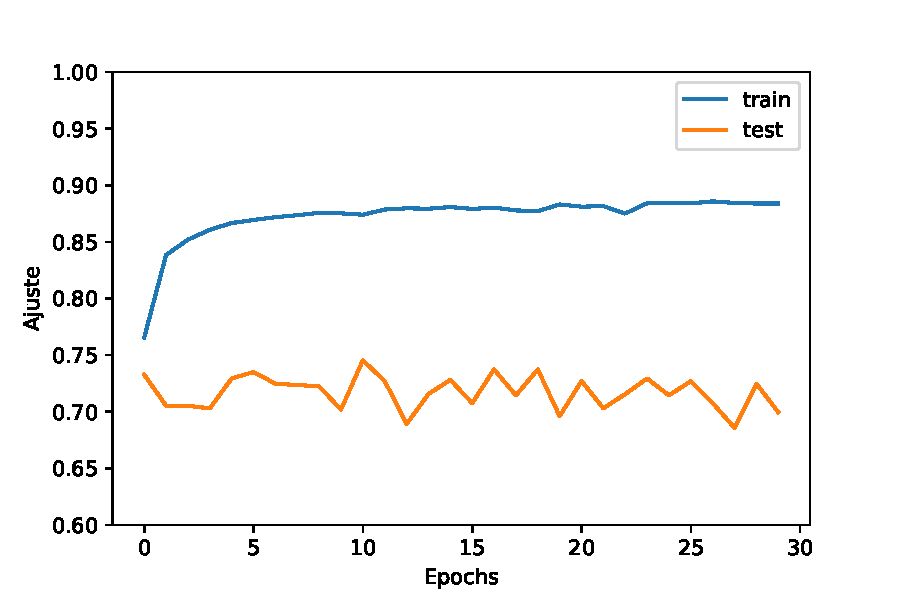
\includegraphics[width=0.6\textwidth]{../Figuras/accuracy_cnn_1.pdf}
	\caption{Ajuste en la Red Neuronal Convolucional Básica}
\end{figure}
\begin{figure}[h!]
	\centering
	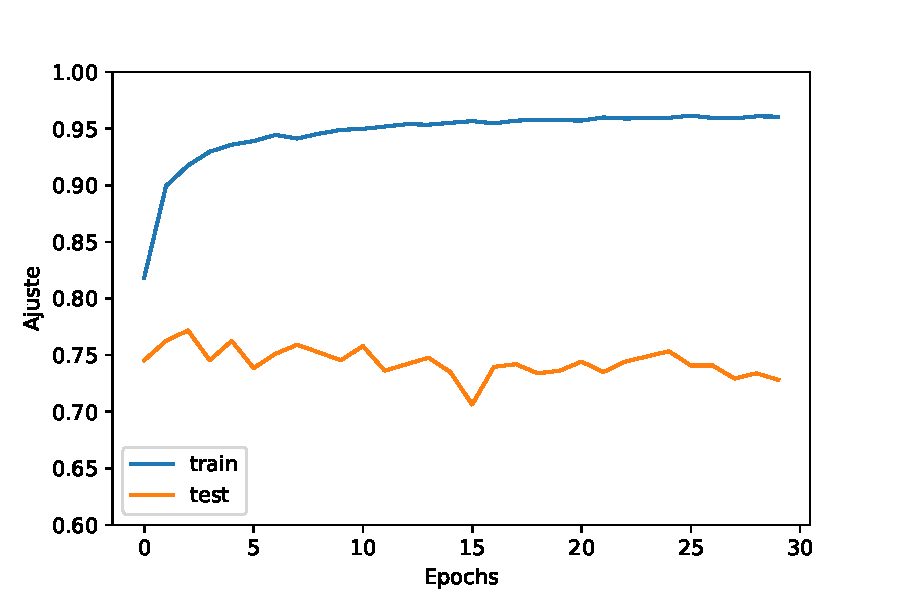
\includegraphics[width=0.6\textwidth]{../Figuras/accuracy_cnn_2.pdf}
	\caption{Ajuste en la Red Neuronal Convolucional Intermedia}
\end{figure}

\end{document}